\chapter{Introduction}

\section{Project Motivation}

% Situation

There is a growing interest in analysing and visualising data generated by users of social networks, which are expanding at an unprecedented rate. Business are looking into utilising these data streams in order to improve their marketing campaigns, refine advertising and better meet their customers needs. Governments of developed countries are also looking into ways of quantifying the wellbeing of their citizens in order to assess effectiveness of local governments and councils. Both tap into the social media in order to determine whether what people are saying is positive or negative. These applications introduce a problem of determining the sentiment of numerous yet short messages, often written in colloquial language. This makes it a very challenging research topic from the perspective of Natural Language Processing and Information Retrieval.

% Complication

There have been attempts to tackle this problem, both in research and industry applications. Researchers have previously either focused on a different domain (e.g. film reviews as in Pang and Lee's paper \cite{PangAndLee}) or only on English (A. Go et al. \cite{TwitterDistantSupervision09}), which accounts for a mere 17.65\% of the global population\footnote{\url{http://en.wikipedia.org/wiki/List_of_countries_by_English-speaking_population}} and only about 50\% of messages posted to Twitter every day.

% Proposal

My goal is to evaluate existing approaches for sentiment classification for languages other than English, focusing initially on four languages: German, Italian, Spanish and Polish. I shall also attempt to utilise crowdsourcing to verify the assumptions of robustness of language classification built into the Twitter API as well as the use of emoticons (e.g. smiley and frowny faces) as labels for training data.

\section{Aims}

Evaluate and discuss the performance of sentiment classification techniques for English, German, Italian, Spanish and Polish tweets. The project shall attempt to achieve the following goals:

\begin{itemize}
  \item Verify the assumption of reliability of language classification provided by Twitter's API.
  \item Verify the assumption that presence of positive or negative emoticons can indeed be used to determine sentiment polarity.
  \item Explore differences in performance of selected algorithms for different languages.
  \item Attempt to explain potential sources of these differences.
  \item Highlight optimal sentiment classification techniques for each language.
\end{itemize}

\section{Related Work}

This project expands upon a number of previously published papers and articles, the summary of which is presented below.

\subsection{Sentiment Analysis}

Multiple papers have been published on sentiment analysis. Some have also explored using social media (and Twitter in particular) as their primary source of data.

Pang and Lee \cite{PangAndLee} present a comprehensive comparison of machine learning algorithms (Na\"ive Bayes, Maximum Entropy and Support Vector Machines) in a fairly narrow domain of film reviews. They evaluate all three algorithms in relation to a number of factors, such as use of unigrams, bigrams or parts of speech tagging. The conclude that whilst Na\"ive Bayes tends to offer inferior performance to Maximum Entropy and SVMs, the differences are typically negligible (1.9pp using unigram presence). They also determine that unigram presence is most effective model and none of the alternatives offered consistently superior performance.

A. Go et al. \cite{TwitterDistantSupervision09} apply the same techniques as Pang and Lee to Twitter messages, but focus solely on English. They also assume emoticons can be used effectively as noisy labels for positive and negative sentiment, quoting previous research by J. Read \cite{Emoticons}, an assumption I verify independently in the Evaluation chapter.

\subsection{Measuring Happiness}

The term ``Gross National Happines'' was coined by Bhutan's former King Jigme Singye Wangchuck in 1972, when he tried to explain his commitment to aligning economic and cultural values of his country.

Since then there have been multiple attempts at mathematically modelling this concept in order to accurately measure and represent society's wellbeing. Due to different factors being taken into account in these models, Gross National Happiness in that form is difficult to compare between multiple countries. Universal approaches, such as the Happy Planet Index (see Figure \ref{fig:happy-planet}), offer a way to do so, but give little insight into how these values change with time (other than on yearly basis).

A. Kramer \cite{GrossNationalHappiness} explores the concept of computational Gross National Happiness index by analysing messages posted by approximately 100 million Facebook users and their activity on the platform. He uses a simplified bag-of-words model where GNH is represented as a difference between the number of positive and negative words in users' status messages. He also validates that positivity of status messages does indeed reflect users' life satisfaction scores. This result has important implications and justifies the need for performing similar analysis for languages other than English.

\begin{figure}[htb]
  \begin{center}
    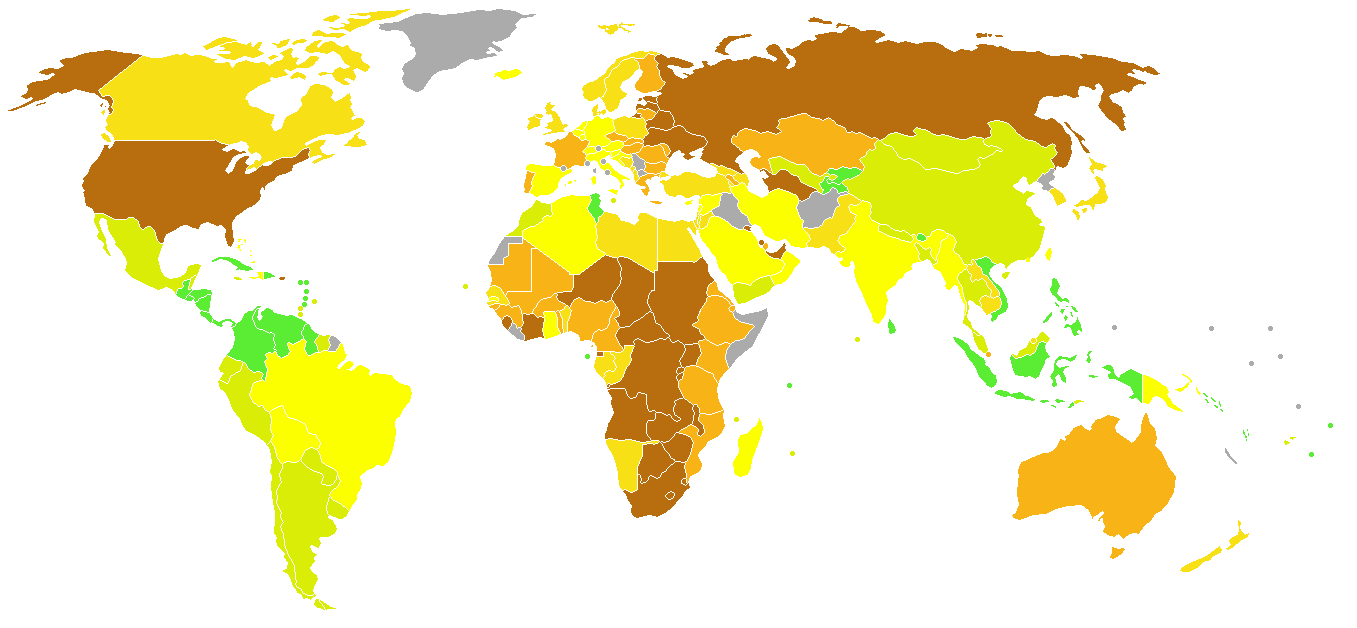
\includegraphics[width=0.8\textwidth]{happy-planet.png}
    \caption{Countries shaded by their position in the Happy Planet Index (2006), where highest-ranked countries are bright green and lowest are brown -- Wikipedia}
    \label{fig:happy-planet}
  \end{center}
\end{figure}

\subsection{Crowdsourcing}

Understanding the limitations of crowdsourcing was considered an important part of this project, given that it was one of the few feasible solutions to verify some of the assumptions made about our data set.

A. Kittur, E. Chi and B. Suh \cite{Crowdsourcing} explain how crowdsourcing using micro-task markets such as Amazon's Mechanical Turk\footnote{\url{http://www.mturk.com}} enables a low time and cost method for collecting user measurements. They offer a number of design recommendations which help achieve more accuracy and higher confidence scores from the use of such methods.

\subsection{Pattern Recognition and Machine Learning}

C. Bishop offers a comprehensive overview of Support Vector Machines and their applications as maximum margin classifiers. He discusses in detail how to model classification problems using linear models in a two-dimensional feature space.

His work has proven invaluable in understanding how Support Vector Machines work and how they can be applied to the problem of sentiment classification.

\subsection{Natural Language Processing}

P. Jackson and I. Moulinier elaborate on the differences between Bayesian information retrieval techniques (such as Na\"ive Bayes classification) and vector space techniques (such as SVMs). This publication provided an algorithmic background required to discuss these techniques in more detail in the Preparation section.

\section{Glossary of Terms}

This subsection explains and clarifies certain terms which are frequently used in subsequent parts of the dissertation.

\begin{itemize}
  \item \textbf{Tweet.} A short message (limited to 140 characters) posted on the social networking and microblogging service called Twitter.
  \item \textbf{Sentiment.} A view of or attitude towards a situation or event; an opinion.
  \item \textbf{Emoticon.} A facial expression pictorially represented by punctuation and letters to alert the respondent to the attitude of statement's author.
  \item \textbf{Application Programming Interface (API).} An interface implemented by a software program to enable interaction with other software, similar to the way a user interface facilitates interaction between humans and computers
  \item \textbf{Gross National Happiness.} An abstract concept of quantifying happiness of citizens in a manner similar to how economy can be quantified using Gross National Product.
  \item \textbf{Crowdsourcing.} Practice of oursourcing tasks to an undefined, large group of people, primarily through the use of online tools.
\end{itemize}